\chapter{Garapenerako ingurune bateratuak - IDEak}\index{IDE}

Eskolak ematen ditudanean beti galdetzen didate ea zein den nik gomendatzen dudan editorea HTML5en garatzeko (edo hobeto esanda, zein den erabiltzen dudan IDEa \index{IDE} - ingelesezko \textit{Integrated Development Environment}, alegia, garapenerako ingurune bateratua). 

Bi ingurune gomendatzen ditut azken bolada honetan (nork daki etorkizunean zein izango den aukera!), \index{VSCode}\href{https://code.visualstudio.com/}{Microsoft VisualStudio Code}\footnote{https://code.visualstudio.com/} eta  \href{https://www.jetbrains.com/idea/}{IntelliJ IDEA}\footnote{https://www.jetbrains.com/idea/}. Egia esan bai bata nola bestea oso IDE onak dira, beraz, garatzaile bakoitzak, bere gustuen arabera, bata edo bestea aukera dezake. Kapitulu honetan bien inguruan oinarri-oinarrizko azalpen bat emango da, lanean hasteko lagundu nahian.

\section{IntelliJ} \index{IntelliJ}

IntelliJ IDEa bi lizentziapean banatzen da. Alde batetik, Ultimate Edition, software pribatiboa. Eta bestetik, Community Edition delakoa, software irekia. Tamalez, Community Edition ezin da erabili gure JavaScript proiektuak kudeatzeko. Zorionez, ikasleak bagara Ultimate edition delakoa dohainik lor dezakegu JetBrains-eko \href{https://www.jetbrains.com/community/education/\#students}{webgunean} eskaera eginez\footnote{https://www.jetbrains.com/community/education/\#students}.

\subsection{Hobespenak}
IntelliJ konfiguratu egin behar da JavaScript proiektuekin lan egiteko lehendabiziko aldian. Zehazki, hobespen hauek:

\begin{enumerate}
    \item \hl{Preferences / Plugins / JavaScript debugger}  (instalatuta eta gaituta dagoela egiaztatu)
    \item \hl{Preferences / Languages and Frameworks / JavaScript / EcmaScript 6} (gaituta dagoela egiaztatu)
    \item \hl{Preferences / Editor / Code Style / JavaScript / Use file extension in module name} (gaituta dagoela egiaztatu)
\end{enumerate}

Jarraian, JavaScript edo HTML proiektu sinple bat sortzeko, \hl{Create a new project / JavaScript} aukeratuko dugu (ikus \ref{fig:intellijsnewjsproject}. irudia).

\begin{figure}[ht]
	\centering
\begin{tikzpicture}
\node[anchor=south west,inner sep=0] (image) at (0,0)
   {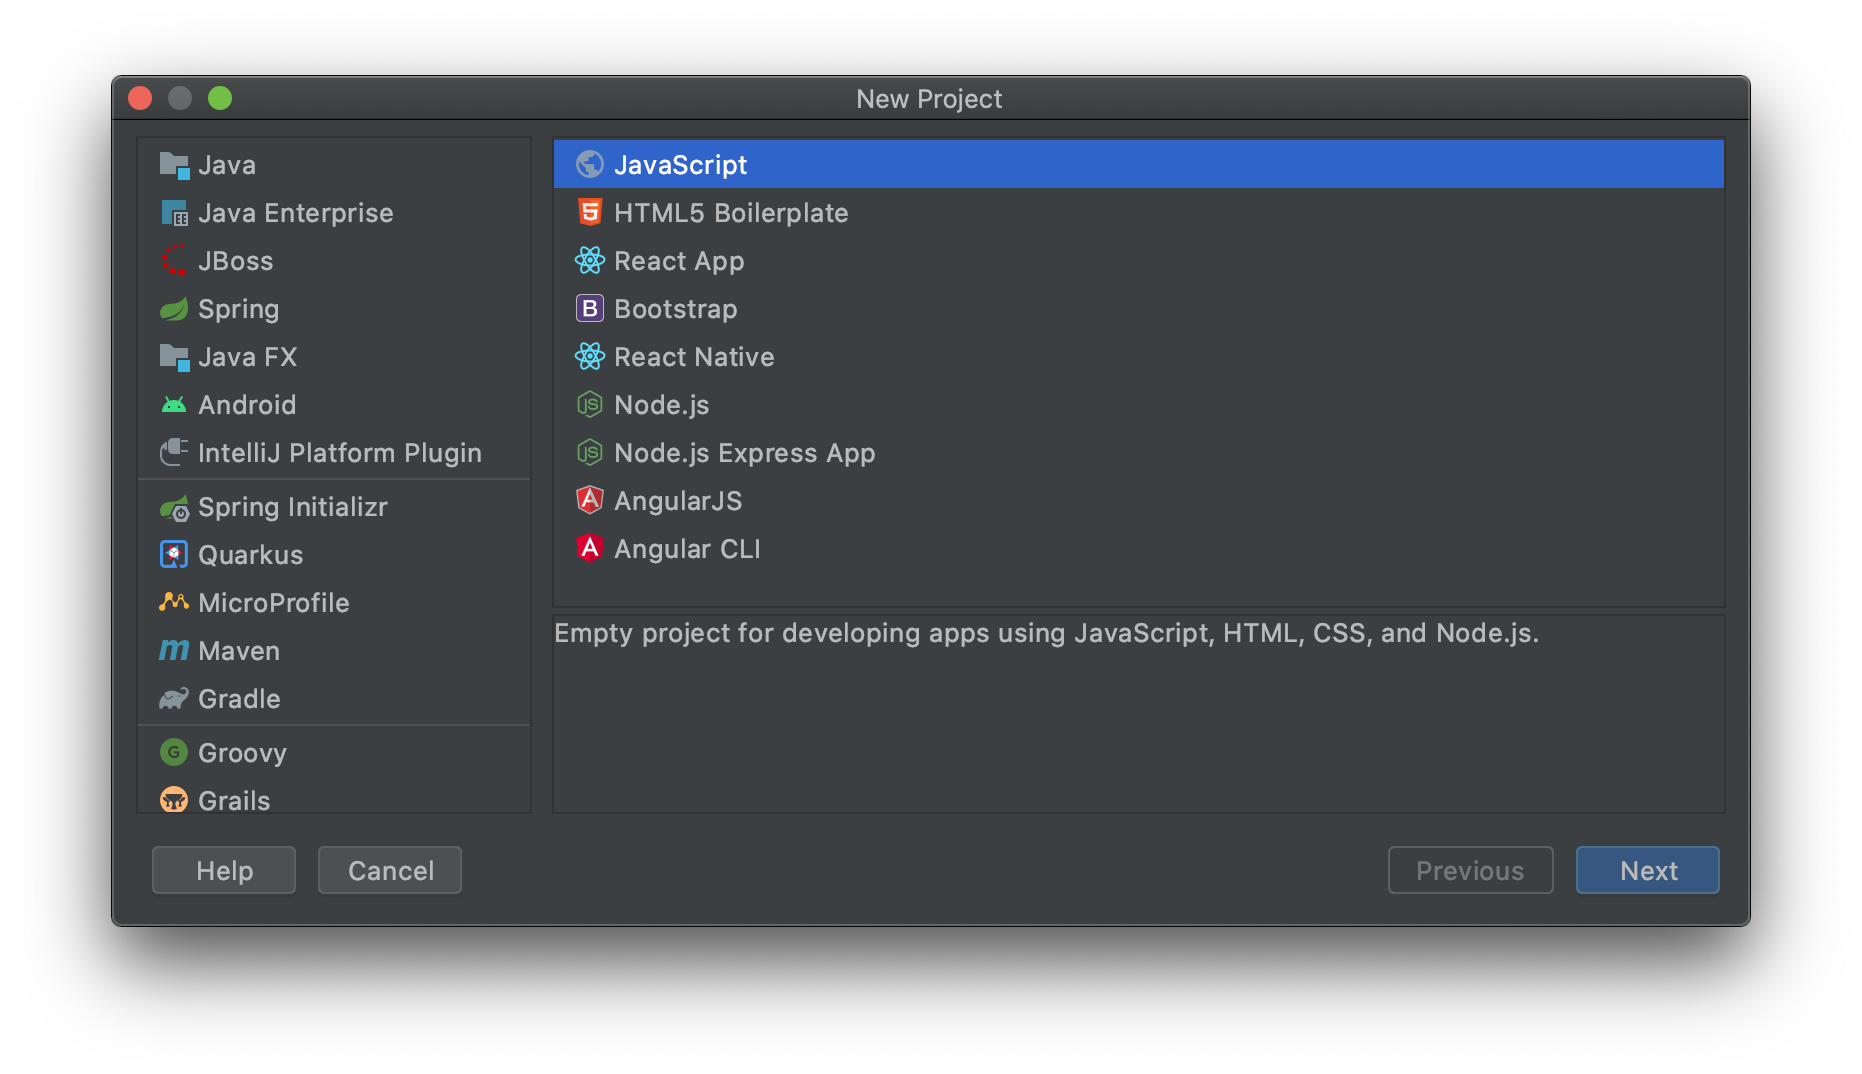
\includegraphics[trim=0cm 0cm 0cm 0cm, clip=true, width=0.75\textwidth]{img/intellijnewproject.png}};
\end{tikzpicture}
\caption{IntelliJ-n JavaScript proiektu mota ezberdinak garatzeko txantiloiak eskuragarri ditugu.}
\label{fig:intellijsnewjsproject}
\end{figure}

Ondoren, proiektuari izena esleitu, zer karpetan gorde nahi dugun zehaztu eta berehala izango dugu proiektuan lan egiteko aukera. 

\begin{figure}[ht]
	\centering
\begin{tikzpicture}
\node[anchor=south west,inner sep=0] (image) at (0,0)
   {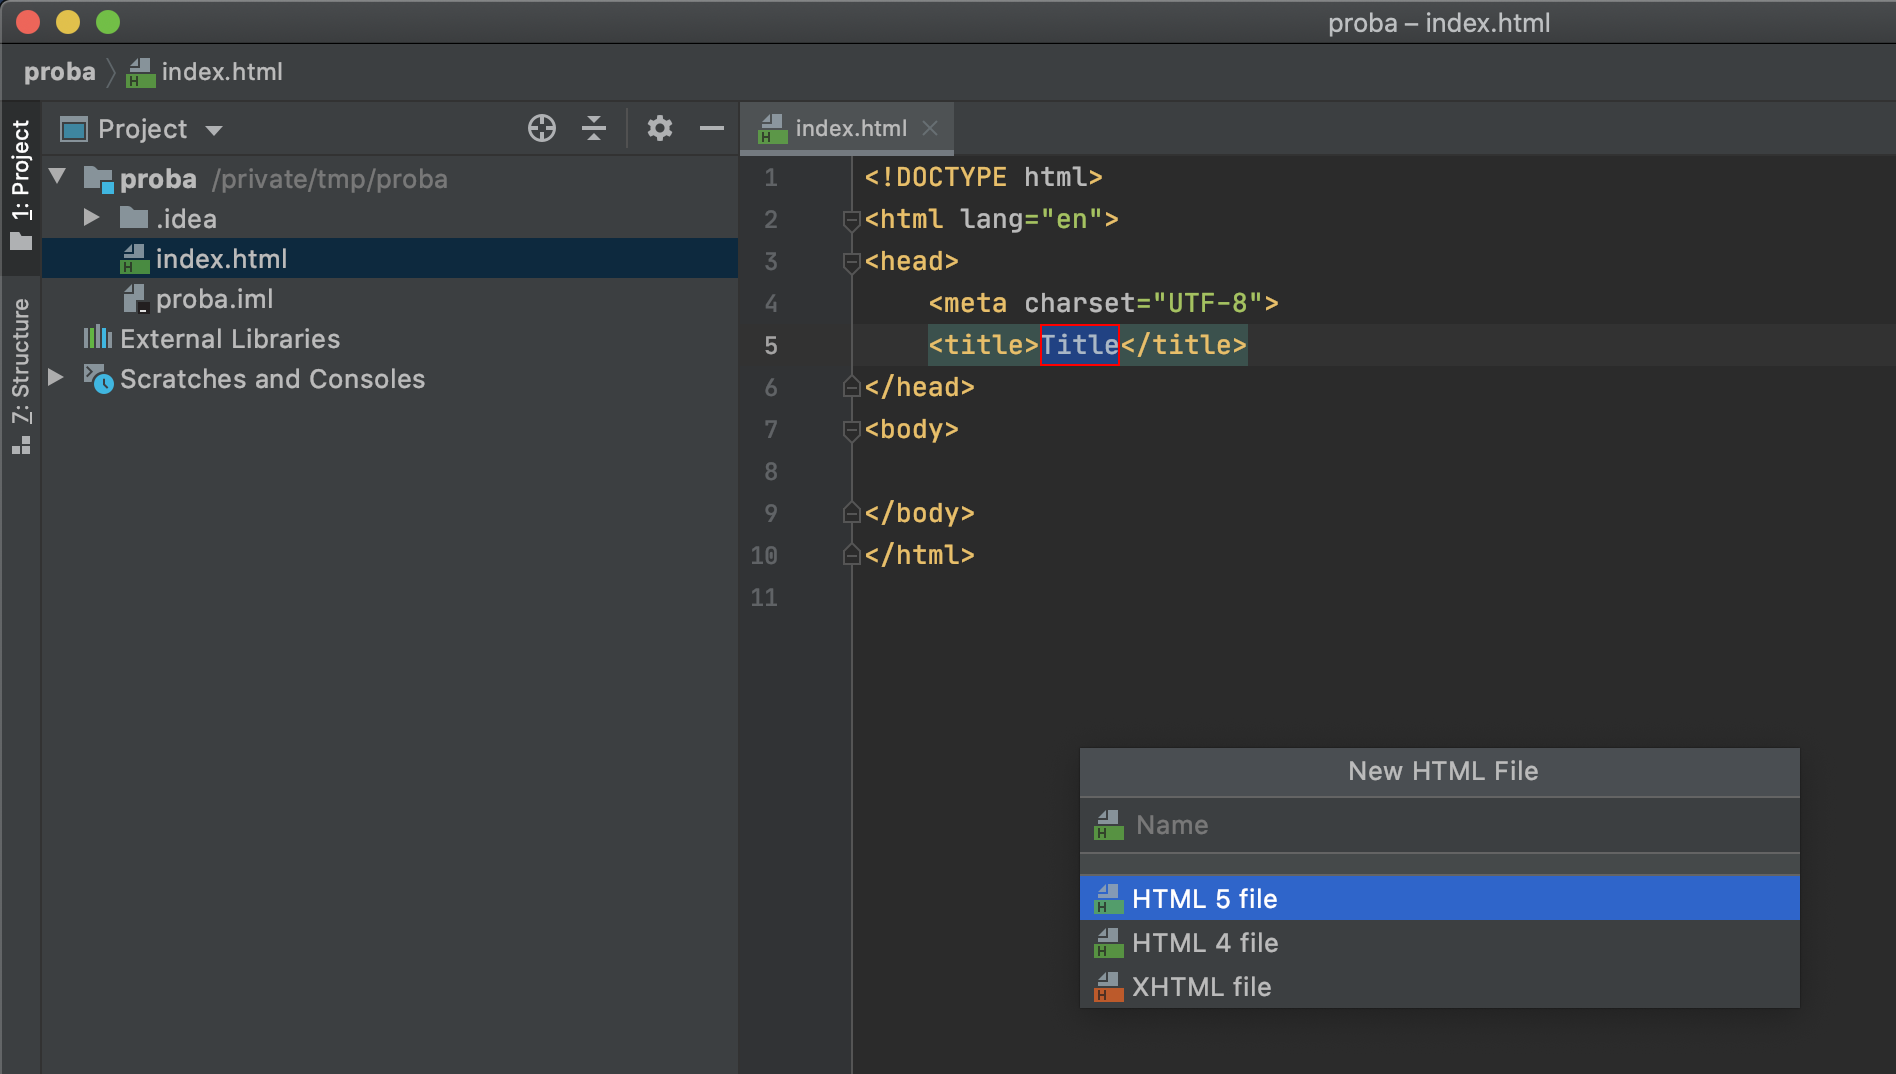
\includegraphics[trim=0cm 0cm 0cm 0cm, clip=true, width=0.75\textwidth]{img/intellijnewproject2.png}};
\end{tikzpicture}
\caption{\hl{File / New HTML file / HTML5} aukeratu eta IntelliJ-k automatikoki HTML5en egindako kode-txantiloi bat sortuko du.}
\label{fig:intellijs}
\end{figure}

Dena ondo konfiguratuta utzi dugula egiaztatzeko, kode hau idatziko dugu, pantailan \hl{canvas} bat sortu eta bertan lauki beltz bat marrazten duena:

\begin{lstlisting}
<!DOCTYPE html>
<html lang="en">
<head><meta charset="UTF-8"><title>Lauki beltza</title>
    <script type="module" src="js/index.js"></script>
</head>
<body><canvas id="arbela" width="640" height="480"></canvas></body></html>
\end{lstlisting}

Orain, seigarren lerroan dagoen \hl{js/index.js} fitxategia eskuz sor dezakegu, baina badago beste metodo azkarrago bat. Fitxategiaren izenaren gainean klik egin eta sagua bertan mantendu, \ref{fig:intellijs3}. irudian dagoen testuinguru-leihoa agertu arte. Bertan \hl{Create File index.js} estekaren gainean sakatu eta IntelliJ-k automatikoki \textit{js/} karpeta sortu eta bertan \textit{index.js} fitxategia gordeko du, hutsik. 


\begin{figure}[ht]
	\centering
\begin{tikzpicture}
\node[anchor=south west,inner sep=0] (image) at (0,0)
   {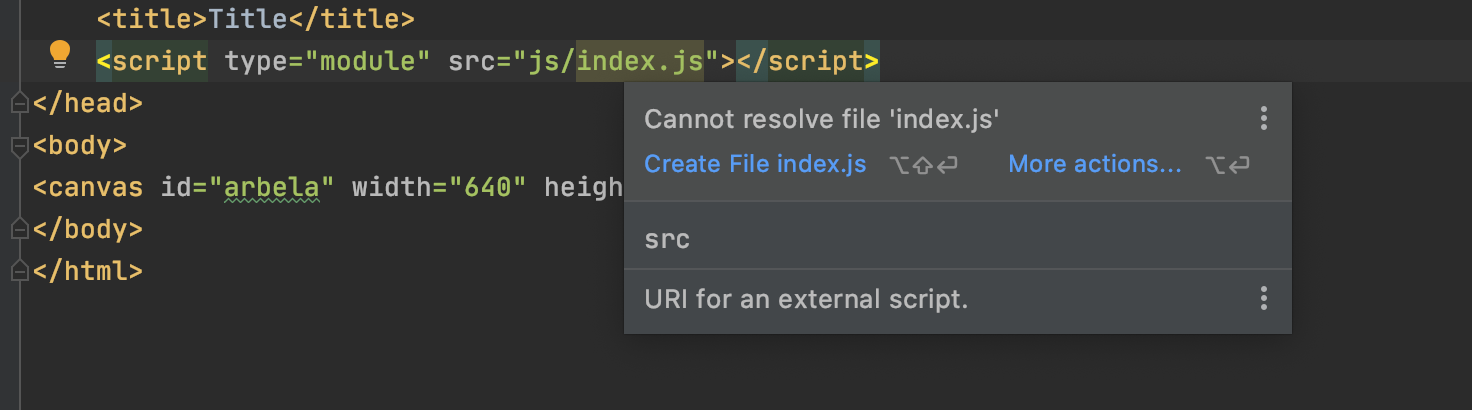
\includegraphics[trim=0cm 0cm 0cm 0cm, clip=true, width=0.75\textwidth]{img/intellijnewproject3.png}};
\end{tikzpicture}
\caption{ IntelliJ-k bonbilla horixka bat erakutsiko digu kodearen ondoan, kodea zuzentzeko gomendio bat duenean.}
\label{fig:intellijs3}
\end{figure}

Orain bai, JS fitxategia honako kodearekin beteko dugu:
\begin{lstlisting}[language=JavaScript,numbers=none]
const canvas = document.getElementById('arbela');
const context = canvas.getContext('2d');
context.fillRect(0,0,50,50);
\end{lstlisting}

Bukatzeko, aplikazioa nabigatzailean probatzeko, IDEak eskaintzen duen nabigatzailearen barran gure gustuko bat hautatuko dugu, adibidez, Chrome. Hautatutako nabigatzailea berehala irekiko da, gure JS aplikazioa bistaratuz, \textit{IntelliJ}-k eskaintzen duen berezko HTTP zerbitzaria erabiliz, portu berezi batean (\ref{fig:emaitza}. irudian 63342 portuan).

\begin{figure}[ht]
	\centering
\begin{tikzpicture}
\node[anchor=south west,inner sep=0] (image) at (0,0)
   {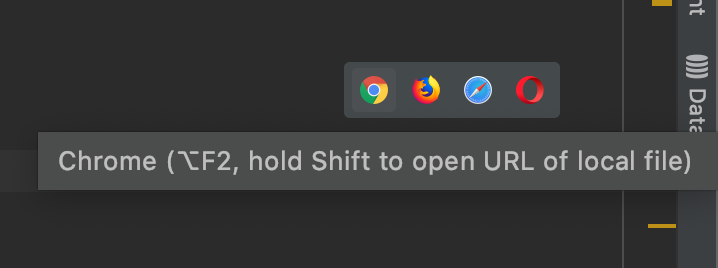
\includegraphics[trim=0cm 0cm 0cm 0cm, clip=true, width=0.75\textwidth]{img/nabigatzaileak.png}};
\end{tikzpicture}
\caption{Alt-F2 sakatuz nabigatzaileen barra agertuko da. Bertan sisteman instalatuta dituzun nabigatzaileen ikurrak ikusiko ditugu. Baten gainean sakatuz, nabigatzaile horretan irekiko da gure aplikazioa.}
\label{fig:nabigatzaileak}
\end{figure}

\begin{figure}[hb]
	\centering
\begin{tikzpicture}[framed]
\node[anchor=south west,inner sep=0] (image) at (0,0)
   {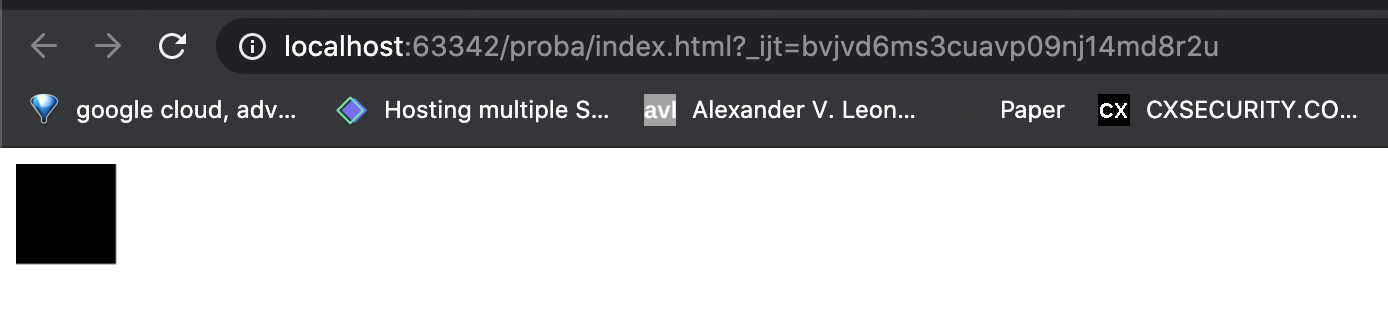
\includegraphics[trim=0cm 0cm 0cm 0cm, clip=true, width=0.75\textwidth]{img/emaitza.png}};
\end{tikzpicture}
\caption{\textit{IntelliJ}-k berezko HTTP zerbitzaria dauka eta bertatik eskainiko du gure JS aplikazioa. URLan ikusten den azken zatia ausazko kate luze bat da, cachearekin arazoak ekiditeko.}
\label{fig:emaitza}
\end{figure}


\section{VSCode} \index{VSCode}

Visual Studio Code (VSCode), Linux, macOS eta Windows-erako eskuragarri dagoen iturburu-kodea editatzeko garapen-ingurune bat da. Microsoft enpresak sortu zuen 2015ean, kode irekiko lizentziapean (MIT). Visual Studio-rekin kodea editatzeaz gain, kodea arazteko, sintaxia nabarmentzeko, automatikoki betetzeko eta hobetzeko (\textit{refactoring})\index{refactoring} aukerak ematen ditu, besteak beste. Are gehiago, ehunka gehigarri eskaintzen ditu, editoreari funtzionaltasun berriak modu erraz batean emateko (adibidez, kodea aztertzeko, beste lengoaia batzuetan programatzeko, editorearen itxura aldatzeko, datu-baseekin integratzeko, etab.)

StackOverflow webgune famatuak urtero argitaratzen duen garatzaileen arteko 2021eko inkestaren arabera, Visual Studio Code izan zen garapen-ingurune ospetsuena (82.000 erantzunen artean, \%70ek VSCode erabiltzen zutela esan zuen).

\begin{figure}[ht]
	\centering
\begin{tikzpicture}[framed]
\node[anchor=south west,inner sep=0] (image) at (0,0)
   {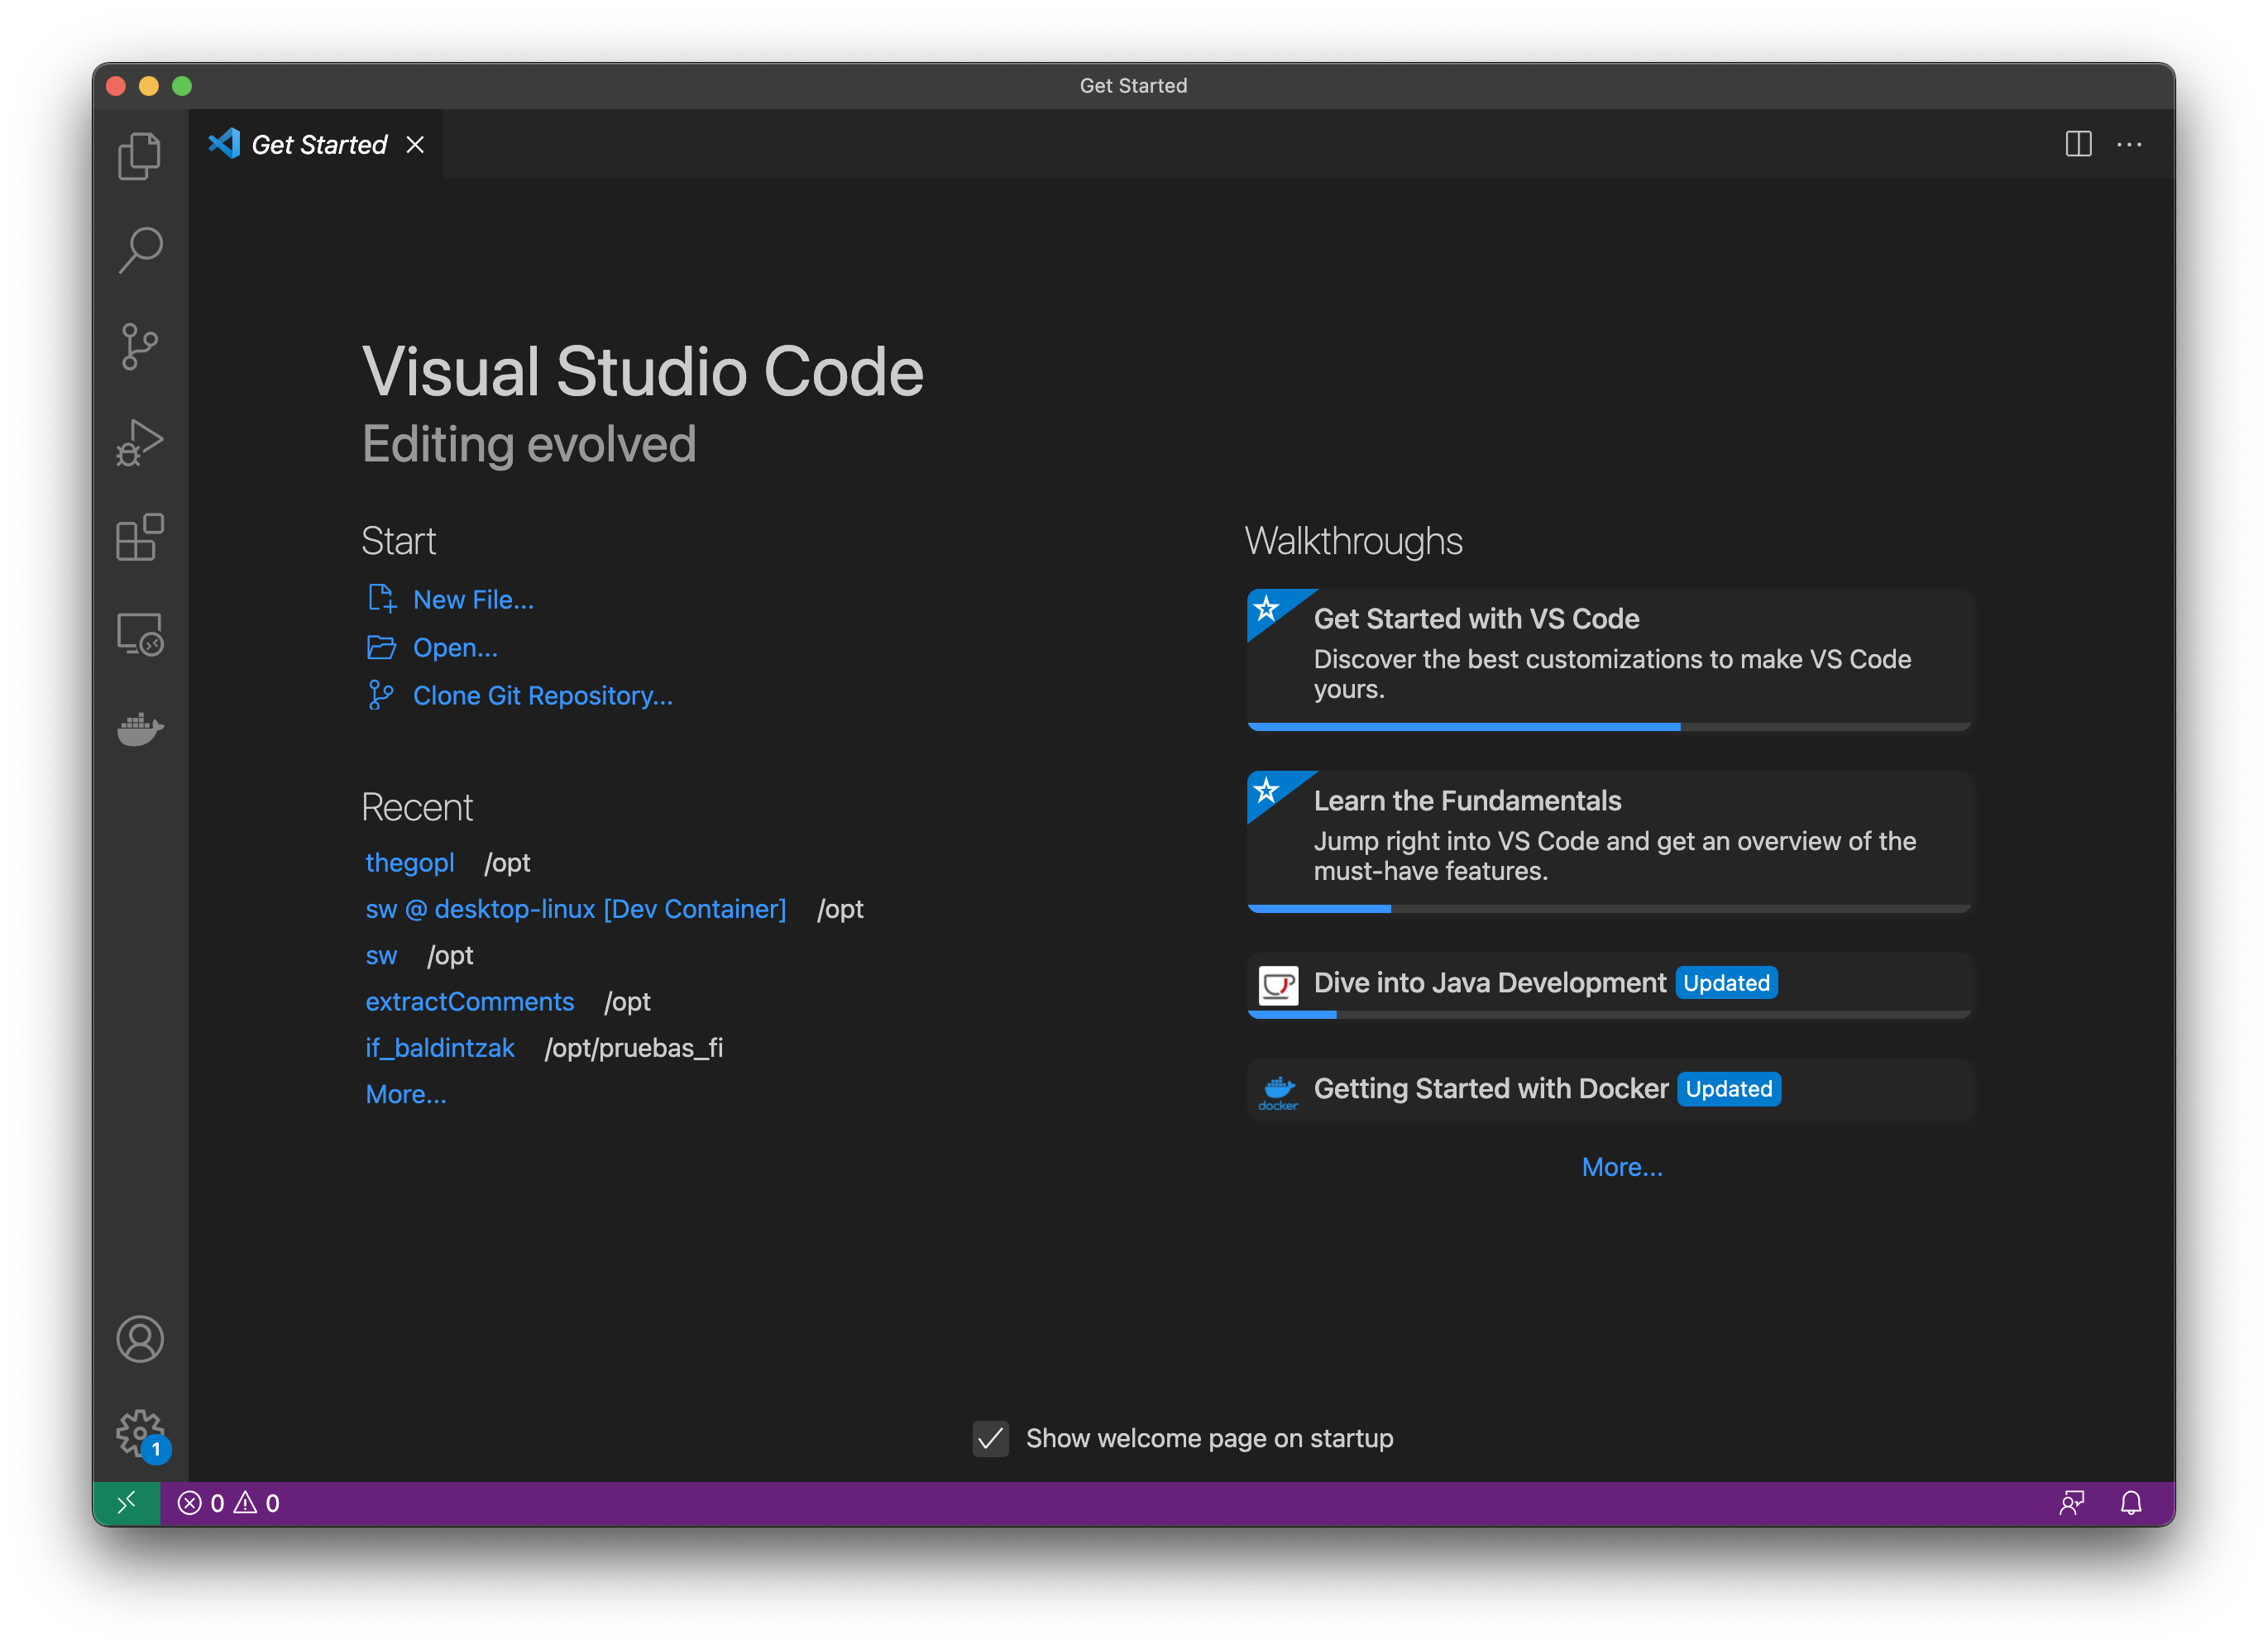
\includegraphics[trim=0cm 0cm 0cm 0cm, clip=true, width=0.75\textwidth]{img/ide/vscode1.png}};
\end{tikzpicture}
\caption{VSCode kode irekiko IDEa sistema eragile erabilienentzat dago eskuragarri.}
\label{fig:vscode1}
\end{figure}


\subsection{Nondik jaitsi}

VSCode-k edozein sistema eragiletarako instalatzailea eskaintzen du \newline 
(\href{https://code.visualstudio.com/}{https://code.visualstudio.com/}).
Instalatu ondoren aplikazioa ireki eta ikusiko dugun lehenengo pantaila \ref{fig:vscode1} irudian ikusten duguna izango da. Bertan, fitxategi berri bat sortu, karpeta ireki edo Git kode-biltegi batetik klonatzeko aukerak ditugu eskuragarri. Aurreko adibidearekin jarraituz, IDE honetan ere oinarrizko HTML eta JavaScript fitxategiak sortuko ditugu, aplikazioarekin lehen urratsak ematen ikasteko.

\subsection{Oinarrizko adibidea}

Lehenengo eta behin, sortu karpeta bat zure disko gogorrean. Horretarako, \mbox{VSCode-n} \textquotedbl{}\textit{Open Folder...}\textquotedbl{} aukeratu eta jarraian irekitzen den pantailan karpeta berria sortzeko aukera izango duzu. Jarraian, HTML fitxategi berri bat sortuko dugu \textquotedbl{}\textit{New File...}\textquotedbl{} botoian sakatuz. Bertan irekitzen den leihotxoan \textquotedbl{}\textit{Text File Built-in}\textquotedbl{} aukeran sakatu. Jarraian, \textquotedbl{}\textit{Select a language}\textquotedbl{} estekan klik egin eta HTML hautatu. 

\begin{figure}[ht]
	\centering
\begin{tikzpicture}[framed]
\node[anchor=south west,inner sep=0] (image) at (0,0)
   {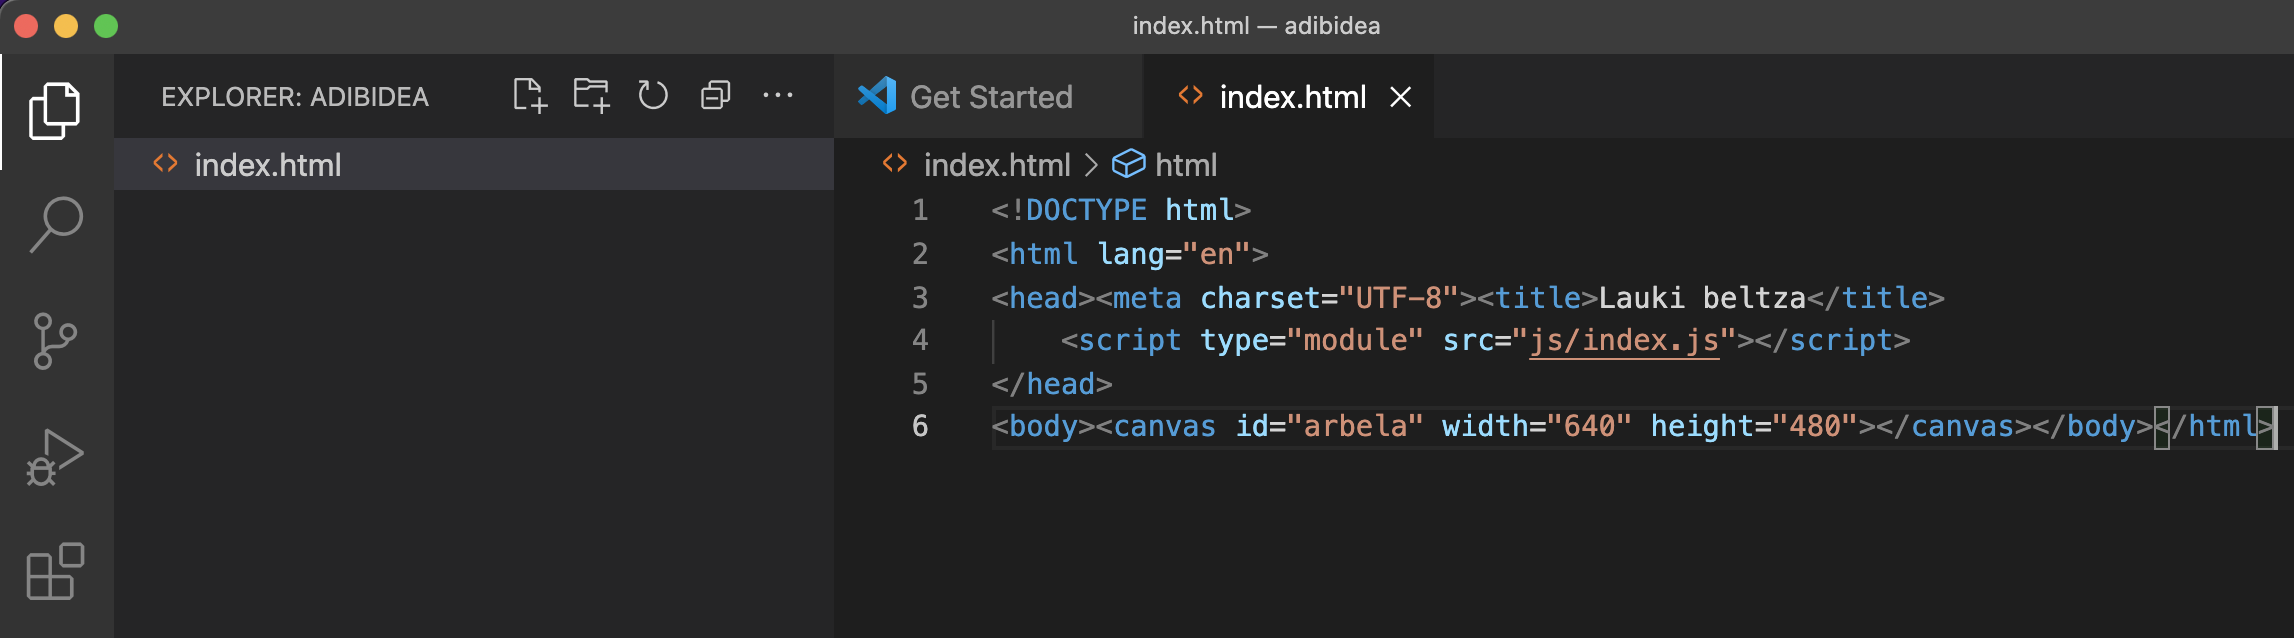
\includegraphics[trim=0cm 0cm 0cm 0cm, clip=true, width=0.75\textwidth]{img/ide/vscode3_1.png}};
\end{tikzpicture}
\caption{VSCode-n, ezkerraldean fitxategien arakatzailea agertuko zaigu. Eskuinaldean editatzen ari garen kodea, sintaxia-nabarmentzearekin.}
\label{fig:vscode3_1}
\end{figure}

\begin{figure}[ht]
	\centering
\begin{tikzpicture}[framed]
\node[anchor=south west,inner sep=0] (image) at (0,0)
   {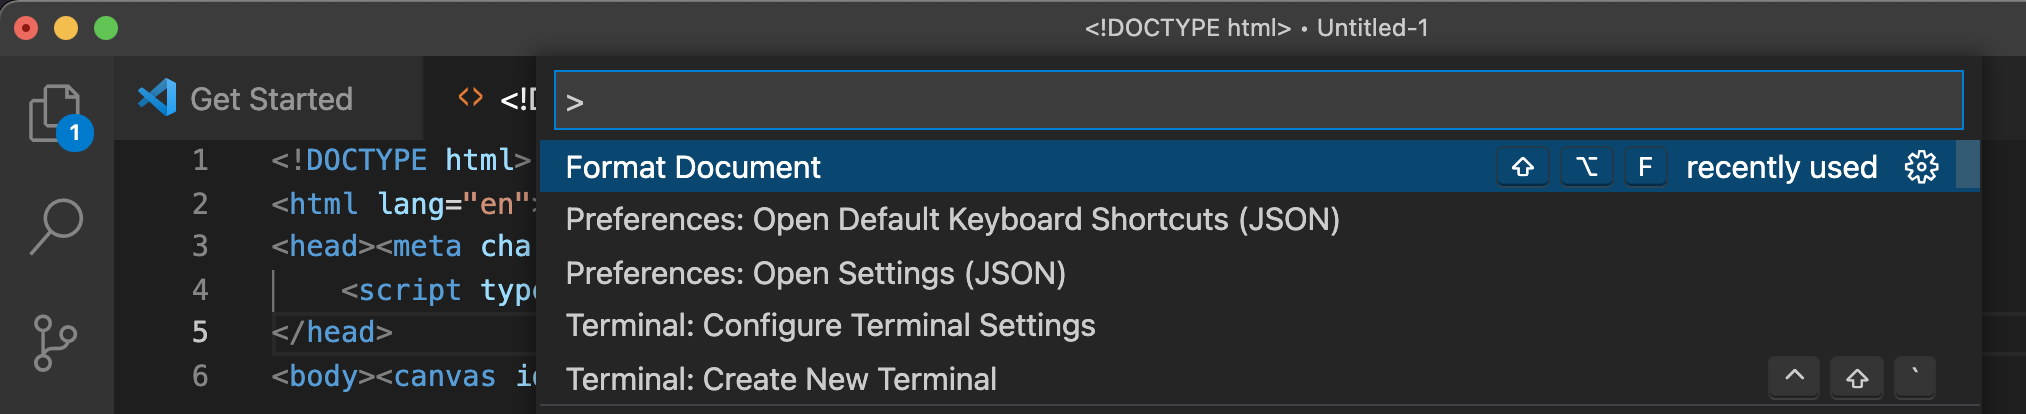
\includegraphics[trim=0cm 0cm 0cm 0cm, clip=true, width=0.75\textwidth]{img/ide/vscode4.png}};
\end{tikzpicture}
\caption{VSCode-k eskaintzen duen komando-paletarekin egin nahi dituzun eragiketak zuzenean idatz ditzakezu, menuetan eragiketa non dagoen bilatu beharrik gabe.}
\label{fig:vscode4}
\end{figure}

Aurreko adibidearen kode bera kopiatu (IntelliJ-en kasuan erabili dugun berbera), eta fitxategia gorde index.html izenarekin, \ref{fig:vscode3_1} irudian dugun pantaila lortuz. Bertan, hiru puntu nabarmenduko ditugu:

\begin{figure}[ht]
	\centering
\begin{tikzpicture}[framed]
\node[anchor=south west,inner sep=0] (image) at (0,0)
   {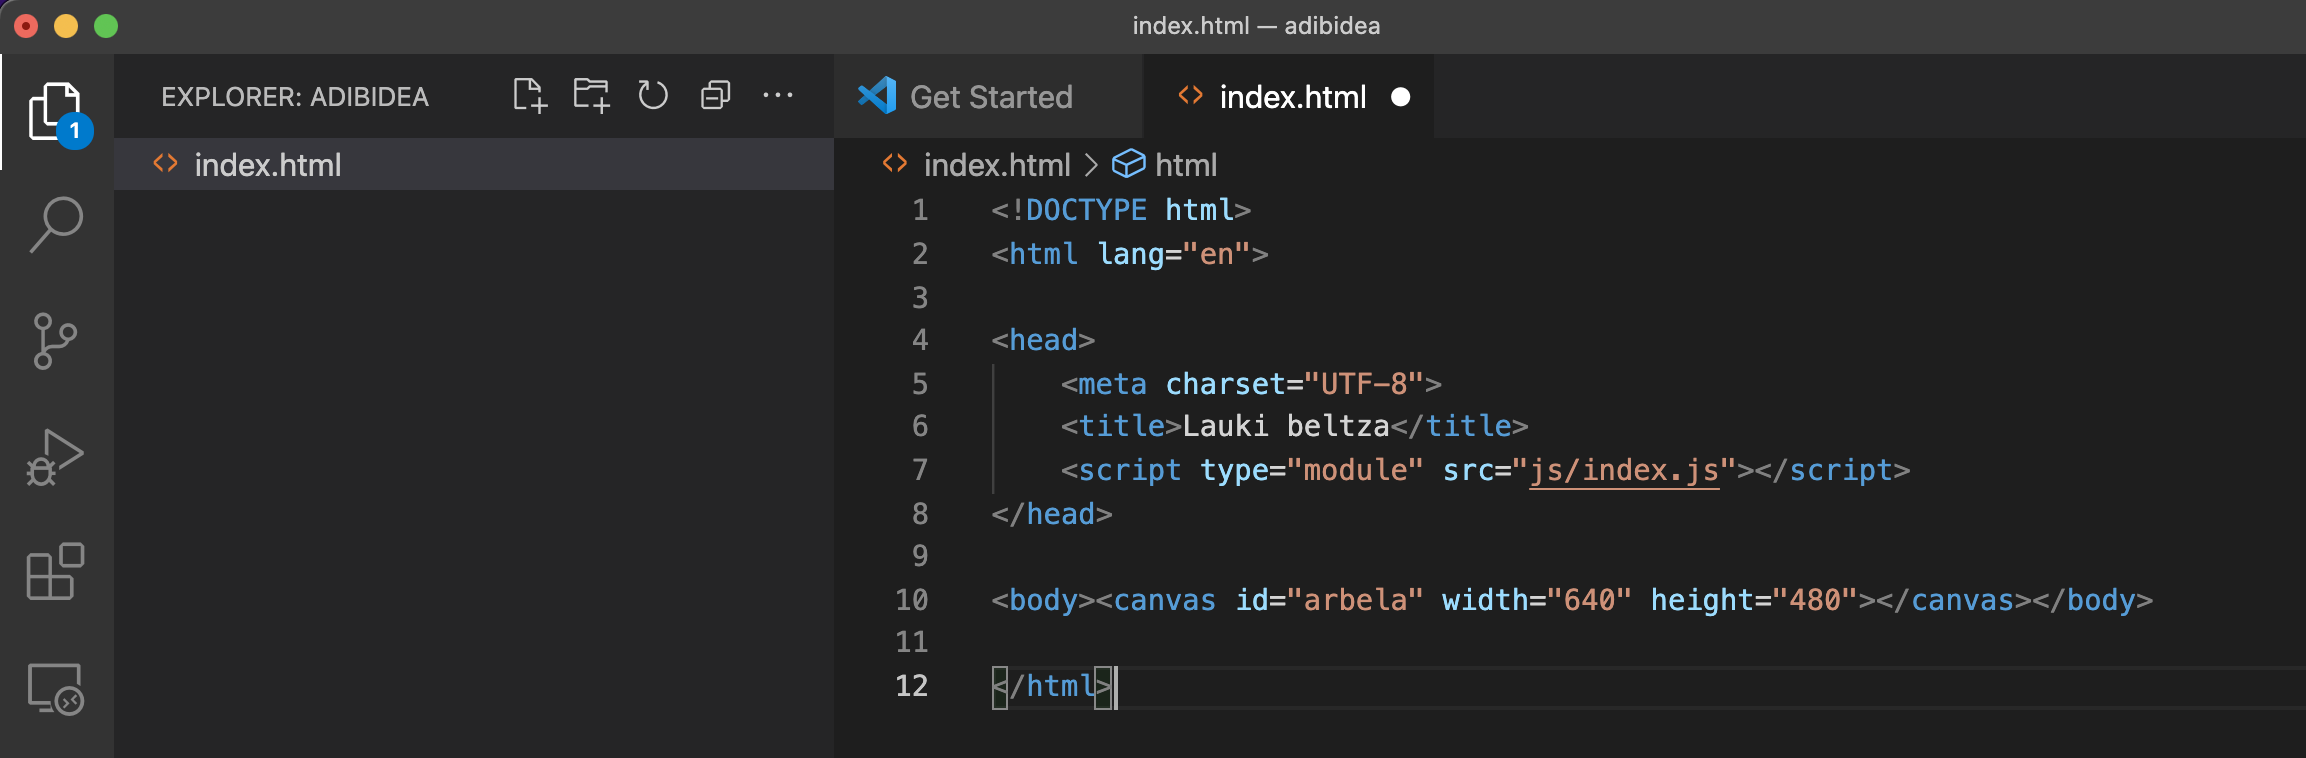
\includegraphics[trim=0cm 0cm 0cm 0cm, clip=true, width=0.75\textwidth]{img/ide/vscode6.png}};
\end{tikzpicture}
\caption{Kodearen formateatze automatikoa aplikatu ondoren, nabarmena da hobekuntza.}
\label{fig:vscode6}
\end{figure}

\begin{itemize}
    \item Aurreko editorean gertatzen zen bezala, \hl{js/index.js} fitxategia sortu gabe dagoenez, bertan sortzeko aukera ematen digu, azpimarratuta agertzen den fitxategiaren izenaren gainean kokatuz eta \textquotedbl{}\textit{Follow Link}\textquotedbl{} aukeratuz. Ondoren, \textquotedbl{}\textit{Create file}\textquotedbl{} botoian sakatu eta fitxategia automatikoki sortuko da.
    
    \item Kodearen sintaxia koloreztatuak balizko akatsak berehala antzematen laguntzen digu.
    
    \item \textit{Copy\&paste} egin dugunez, kodearen formatua ez da hoberena. Hori konpontzeko \hl{Control-Shift-P} sakatuko dugu VSCode-n aginduak sartzeko \newline \textit{Command-Palette} deritzon leihoa irekitzeko (\ref{fig:vscode4} irudia). Bertan gaudelarik, \textquotedbl{}\textit{Format Document}\textquotedbl{} hautatuko dugu, kodeari formatua emateko. Emaitza \ref{fig:vscode6} irudian ikus daiteke.    
\end{itemize}

\begin{alertinfo}{Visual Studio Code eta laster-teklak}\index{cheatsheet}\index{laster-teklak}
VSCode-k erabiltzen dituen laster-teklak oso baliagarriak dira IDE honek eskaintzen dituen milaka funtzioen artean erabilienak berehala exekutatu ahal izateko. Arazoa da laster-tekla horiek ere asko direla. Horrez gain, ezberdinak izango dira erabiltzailearen sistema eragilearen arabera. Arazo hauek konpontzeko VSCode-k \textit{txuleta} (\textit{cheatsheet}) batzuk eskaintzen ditu, Linux\footnote{\href{https://code.visualstudio.com/shortcuts/keyboard-shortcuts-linux.pdf}{https://code.visualstudio.com/shortcuts/keyboard-shortcuts-linux.pdf}}, macOS\footnote{\href{https://code.visualstudio.com/shortcuts/keyboard-shortcuts-macos.pdf}{https://code.visualstudio.com/shortcuts/keyboard-shortcuts-macos.pdf}} eta Windows  \footnote{\href{https://code.visualstudio.com/shortcuts/keyboard-shortcuts-windows.pdf}{https://code.visualstudio.com/shortcuts/keyboard-shortcuts-windows.pdf}} sistemetarako.

\end{alertinfo}


